
\documentclass{article}[14pt]
\usepackage{multicol, enumerate, enumitem, hyperref, color, soul, setspace, parskip, fancyhdr, amssymb, amsthm, amsmath, bbm, latexsym, units, mathtools}
\everymath{\displaystyle}
\usepackage[headsep=0.5cm,headheight=0cm, left=1 in,right= 1 in,top= 1 in,bottom= 1 in]{geometry}
\pagestyle{fancy}
\lhead{}
\chead{Answer Key for Module\,7\,-\,Rational\,Functions Version C}
\rhead{}
\lfoot{Summer\,C\,2020}
\cfoot{}
\rfoot{}
\begin{document}
\textbf{This key should allow you to understand why you choose the option you did (beyond just getting a question right or wrong). \href{https://xronos.clas.ufl.edu/mac1105spring2020/courseDescriptionAndMisc/Exams/LearningFromResults}{More instructions on how to use this key can be found here}.}

\textbf{If you have a suggestion to make the keys better, \href{https://forms.gle/CZkbZmPbC9XALEE88}{please fill out the short survey here}.}

\textit{Note: This key is auto-generated and may contain issues and/or errors. The keys are reviewed after each exam to ensure grading is done accurately. If there are issues (like duplicate options), they are noted in the offline gradebook. The keys are a work-in-progress to give students as many resources to improve as possible.}

\rule{\textwidth}{0.4pt}

31. Solve the rational equation below. Then, choose the interval(s) that the solution(s) belongs to.
$$ \frac{-9}{5x + 6} + 5 = \frac{-4}{-45x -54} $$ 
The solution is $ x = -0.822 $ 

\begin{enumerate}[label=\Alph*.] 
\item $ x \in [-0.82,0.18] $ 

 * $x = -0.822$, which is the correct option. 
\item $ x_1 \in [-0.95, -0.8] \text{ and } x_2 \in [0,3] $ 

 $x = -0.822 \text{ and } x = 1.578$, which corresponds to getting the correct solution and believing there should be a second solution to the equation. 
\item $ x \in [1.51,1.62] $ 

 $x = 1.578$, which corresponds to not distributing the factor $5x + 6$ correctly when trying to eliminate the fraction. 
\item $ \text{All solutions lead to invalid or complex values in the equation.} $ 

 This corresponds to thinking $x = -0.822$ leads to dividing by zero in the original equation, which it does not. 
\item $ x_1 \in [-1.11, -0.84] \text{ and } x_2 \in [-7,0] $ 

 $x = -1.000 \text{ and } x = -0.822$, which corresponds to getting the correct solution and believing there should be a second solution to the equation. 
\end{enumerate} 
 
General Comments: Distractors are different based on the number of solutions. Remember that after solving, we need to make sure our solution does not make the original equation divide by zero!

-----------------------------------------------

32. Determine the domain of the function below.
$$ f(x) = \frac{4}{12x^{2} +3 x -15} $$ 
The solution is $ \text{All Real numbers except } x = -1.250 \text{ and } x = 1.000. $ 

\begin{enumerate}[label=\Alph*.] 
\item $ \text{All Real numbers except } x = a, \text{ where } a \in [-21.3, -19.1] $ 

 All Real numbers except $x = -20.000$, which corresponds to removing a distractor value from the denominator. 
\item $ \text{All Real numbers except } x = a \text{ and } x = b, \text{ where } a \in [-21.3, -19.1] \text{ and } b \in [8.7, 9.2] $ 

 All Real numbers except $x = -20.000$ and $x = 9.000$, which corresponds to not factoring the denominator correctly. 
\item $ \text{All Real numbers.} $ 

 This corresponds to thinking the denominator has complex roots or that rational functions have a domain of all Real numbers. 
\item $ \text{All Real numbers except } x = a, \text{ where } a \in [-1.4, -0.5] $ 

 All Real numbers except $x = -1.250$, which corresponds to removing only 1 value from the denominator. 
\item $ \text{All Real numbers except } x = a \text{ and } x = b, \text{ where } a \in [-1.4, -0.5] \text{ and } b \in [0.7, 1.7] $ 

 All Real numbers except $x = -1.250$ and $x = 1.000$, which is the correct option. 
\end{enumerate} 
 
General Comments: The new domain is the intersection of the previous domains.

-----------------------------------------------

33. Choose the equation of the function graphed below.
\begin{center} 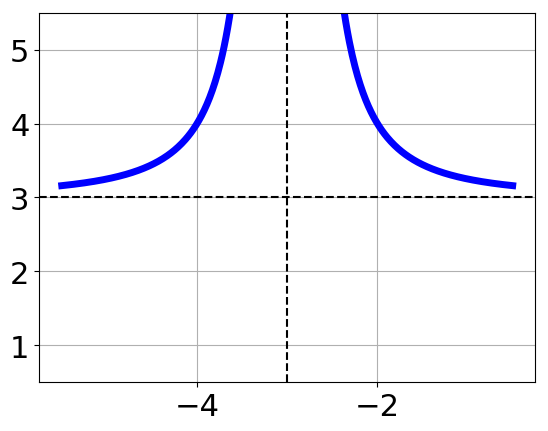
\includegraphics[width=0.3\textwidth]{../Figures/rationalGraphToEquationC.png} \end{center} 

The solution is $ f(x) = \frac{1}{(x + 1)^2} - 1 $ 

\begin{enumerate}[label=\Alph*.] 
\item $ f(x) = \frac{-1}{(x - 1)^2} - 1 $ 

 Corresponds to using the general form $f(x) = \frac{a}{(x+h)^2}+k$ and the opposite leading coefficient. 
\item $ f(x) = \frac{-1}{x - 1} - 1 $ 

 Corresponds to thinking the graph was a shifted version of $\frac{1}{x}$, using the general form $f(x) = \frac{a}{(x+h)^2}+k$, and the opposite leading coefficient. 
\item $ f(x) = \frac{1}{x + 1} - 1 $ 

 Corresponds to thinking the graph was a shifted version of $\frac{1}{x}$. 
\item $ f(x) = \frac{1}{(x + 1)^2} - 1 $ 

 This is the correct option. 
\item $ \text{None of the above} $ 

 This corresponds to believing the vertex of the graph was not correct. 
\end{enumerate} 
 
General Comments: Remember that the general form of a basic rational equation is $ f(x) = \frac{a}{(x-h)^n} + k$, where $a$ is the leading coefficient (and in this case, we assume is either $1$ or $-1$), $n$ is the degree (in this case, either $1$ or $2$), and $(h, k)$ is the intersection of the asymptotes.

-----------------------------------------------

34. Choose the graph of the equation below.
$$ f(x) = \frac{-1}{(x + 1)^2} + 2 $$ 

 
 The solution is  
 \begin{center} 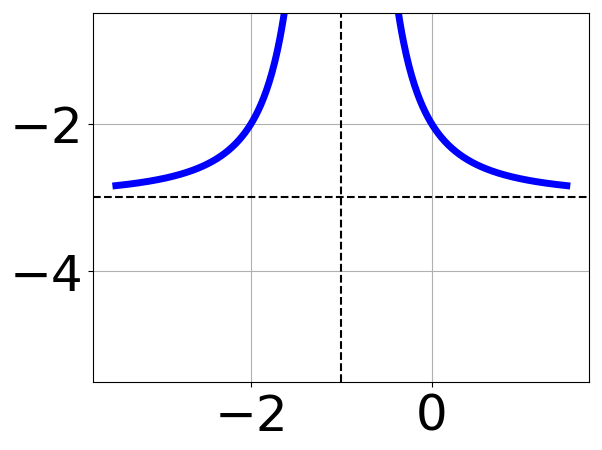
\includegraphics[width=0.3\textwidth]{../Figures/rationalEquationToGraphCB.png} \end{center}\begin{tabular}{|c|c|} 
\hline 
 & \tabularnewline 
 \textbf{A.} 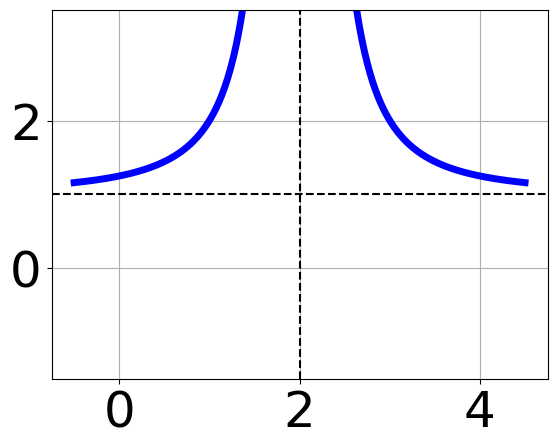
\includegraphics[width=0.3\textwidth]{../Figures/rationalEquationToGraphCA.png} & \textbf{B.} 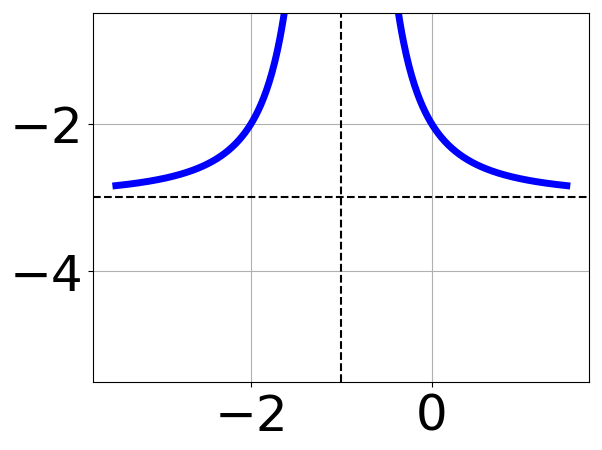
\includegraphics[width=0.3\textwidth]{../Figures/rationalEquationToGraphCB.png} \tabularnewline 
\hline 
 & \tabularnewline 
 \textbf{C.} 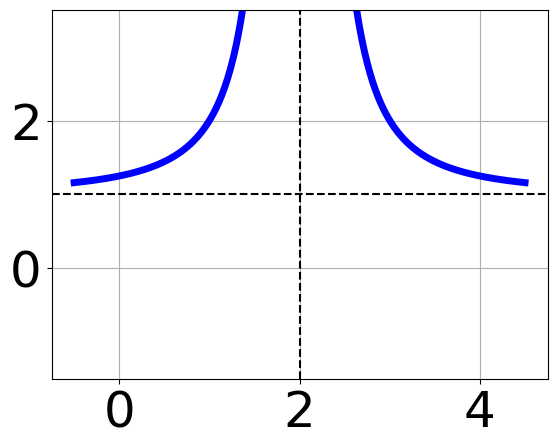
\includegraphics[width=0.3\textwidth]{../Figures/rationalEquationToGraphCC.png} & \textbf{D.} 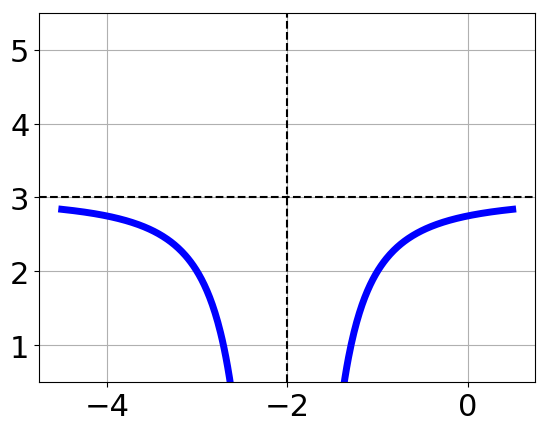
\includegraphics[width=0.3\textwidth]{../Figures/rationalEquationToGraphCD.png} \tabularnewline 
\hline 
 E. None of the figures above. & \tabularnewline 
\hline 
 \end{tabular} 
 
General Comments: Remember that the general form of a basic rational equation is $ f(x) = \frac{a}{(x-h)^n} + k$, where $a$ is the leading coefficient (and in this case, we assume is either $1$ or $-1$), $n$ is the degree (in this case, either $1$ or $2$), and $(h, k)$ is the intersection of the asymptotes.

-----------------------------------------------

35. Solve the rational equation below. Then, choose the interval(s) that the solution(s) belongs to.
$$ \frac{-3x}{3x -3} + \frac{-6x^{2}}{12x^{2} -33 x + 21} = \frac{5}{4x -7} $$ 
The solution is $ \text{There are two solutions: } x = 1.095 \text{ and } x = -0.761 $ 

\begin{enumerate}[label=\Alph*.] 
\item $ x \in [-0.8,0.57] $ 

  
\item $ \text{All solutions lead to invalid or complex values in the equation.} $ 

  
\item $ x_1 \in [0.11, 1.74] \text{ and } x_2 \in [-5.9,0.2] $ 

 * $x = 1.095 \text{ and } x = -0.761$, which is the correct option. 
\item $ x_1 \in [0.11, 1.74] \text{ and } x_2 \in [-0.3,2.4] $ 

  
\item $ x \in [1.58,2.82] $ 

  
\end{enumerate} 
 
General Comments: Distractors are different based on the number of solutions. Remember that after solving, we need to make sure our solution does not make the original equation divide by zero!

-----------------------------------------------

31. Choose the graph of the equation below.
$$ f(x) = \frac{-1}{x + 2} + 3 $$ 

 
 The solution is  
 \begin{center} 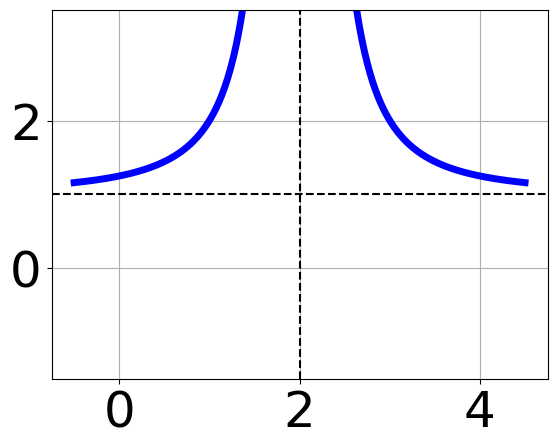
\includegraphics[width=0.3\textwidth]{../Figures/rationalEquationToGraphCA.png} \end{center}\begin{tabular}{|c|c|} 
\hline 
 & \tabularnewline 
 \textbf{A.} 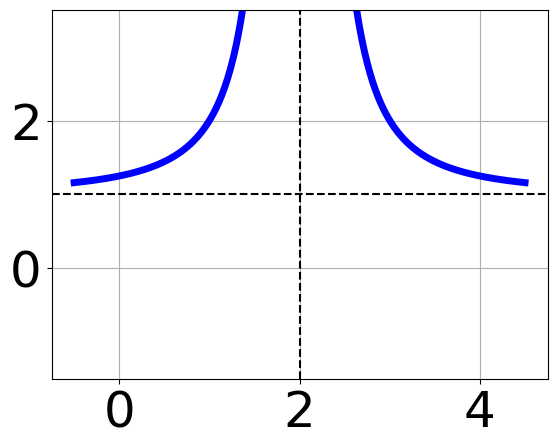
\includegraphics[width=0.3\textwidth]{../Figures/rationalEquationToGraphCA.png} & \textbf{B.} 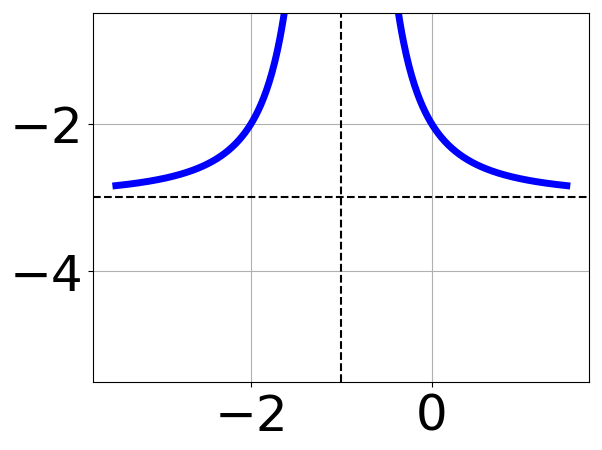
\includegraphics[width=0.3\textwidth]{../Figures/rationalEquationToGraphCB.png} \tabularnewline 
\hline 
 & \tabularnewline 
 \textbf{C.} 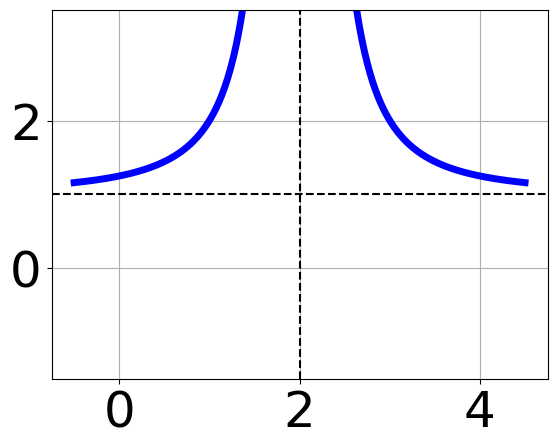
\includegraphics[width=0.3\textwidth]{../Figures/rationalEquationToGraphCC.png} & \textbf{D.} 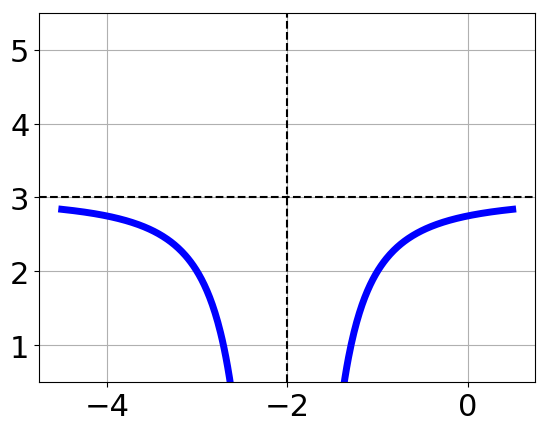
\includegraphics[width=0.3\textwidth]{../Figures/rationalEquationToGraphCD.png} \tabularnewline 
\hline 
 E. None of the figures above. & \tabularnewline 
\hline 
 \end{tabular} 
 
General Comments: Remember that the general form of a basic rational equation is $ f(x) = \frac{a}{(x-h)^n} + k$, where $a$ is the leading coefficient (and in this case, we assume is either $1$ or $-1$), $n$ is the degree (in this case, either $1$ or $2$), and $(h, k)$ is the intersection of the asymptotes.

-----------------------------------------------

32. Solve the rational equation below. Then, choose the interval(s) that the solution(s) belongs to.
$$ \frac{5x}{6x -2} + \frac{-6x^{2}}{-24x^{2} +38 x -10} = \frac{2}{-4x + 5} $$ 
The solution is $ \text{There are two solutions: } x = 0.715 \text{ and } x = -0.215 $ 

\begin{enumerate}[label=\Alph*.] 
\item $ x \in [1.15,2.01] $ 

  
\item $ x_1 \in [0.03, 1.17] \text{ and } x_2 \in [-2.17,0.1] $ 

 * $x = 0.715 \text{ and } x = -0.215$, which is the correct option. 
\item $ \text{All solutions lead to invalid or complex values in the equation.} $ 

  
\item $ x \in [-0.23,0.12] $ 

  
\item $ x_1 \in [0.03, 1.17] \text{ and } x_2 \in [0.13,1.45] $ 

  
\end{enumerate} 
 
General Comments: Distractors are different based on the number of solutions. Remember that after solving, we need to make sure our solution does not make the original equation divide by zero!

-----------------------------------------------

33. Solve the rational equation below. Then, choose the interval(s) that the solution(s) belongs to.
$$ \frac{-2}{-7x -6} + 5 = \frac{8}{-49x -42} $$ 
The solution is $ x = -0.947 $ 

\begin{enumerate}[label=\Alph*.] 
\item $ x \in [0.39,0.83] $ 

 $x = 0.767$, which corresponds to not distributing the factor $-7x -6$ correctly when trying to eliminate the fraction. 
\item $ x_1 \in [-1.14, -0.72] \text{ and } x_2 \in [0,1] $ 

 $x = -0.947 \text{ and } x = 0.767$, which corresponds to getting the correct solution and believing there should be a second solution to the equation. 
\item $ \text{All solutions lead to invalid or complex values in the equation.} $ 

 This corresponds to thinking $x = -0.947$ leads to dividing by zero in the original equation, which it does not. 
\item $ x \in [-0.95,0.05] $ 

 * $x = -0.947$, which is the correct option. 
\item $ x_1 \in [-1.36, -1.01] \text{ and } x_2 \in [-2,0] $ 

 $x = -1.143 \text{ and } x = -0.947$, which corresponds to getting the correct solution and believing there should be a second solution to the equation. 
\end{enumerate} 
 
General Comments: Distractors are different based on the number of solutions. Remember that after solving, we need to make sure our solution does not make the original equation divide by zero!

-----------------------------------------------

34. Determine the domain of the function below.
$$ f(x) = \frac{6}{20x^{2} -4 x -24} $$ 
The solution is $ \text{All Real numbers except } x = -1.000 \text{ and } x = 1.200. $ 

\begin{enumerate}[label=\Alph*.] 
\item $ \text{All Real numbers except } x = a, \text{ where } a \in [-3.4, 0.1] $ 

 All Real numbers except $x = -1.000$, which corresponds to removing only 1 value from the denominator. 
\item $ \text{All Real numbers except } x = a \text{ and } x = b, \text{ where } a \in [-3.4, 0.1] \text{ and } b \in [0.3, 2] $ 

 All Real numbers except $x = -1.000$ and $x = 1.200$, which is the correct option. 
\item $ \text{All Real numbers.} $ 

 This corresponds to thinking the denominator has complex roots or that rational functions have a domain of all Real numbers. 
\item $ \text{All Real numbers except } x = a \text{ and } x = b, \text{ where } a \in [-17.5, -15.8] \text{ and } b \in [29.3, 30.4] $ 

 All Real numbers except $x = -16.000$ and $x = 30.000$, which corresponds to not factoring the denominator correctly. 
\item $ \text{All Real numbers except } x = a, \text{ where } a \in [-17.5, -15.8] $ 

 All Real numbers except $x = -16.000$, which corresponds to removing a distractor value from the denominator. 
\end{enumerate} 
 
General Comments: The new domain is the intersection of the previous domains.

-----------------------------------------------


\end{document}

